\documentclass[11pt]{article}
\usepackage[margin=1in]{geometry}
\usepackage{amsmath,amssymb}
\usepackage{booktabs,enumitem,xcolor,array,tabularx,graphicx,float,longtable}
\usepackage{microtype}
\usepackage[most]{tcolorbox}
\usepackage[colorlinks=true,linkcolor=blue!50!black,citecolor=blue!50!black,urlcolor=blue!50!black]{hyperref}
\newcolumntype{Y}{>{\raggedright\arraybackslash}X}
\newcolumntype{P}[1]{>{\raggedright\arraybackslash}p{#1}}
\setlength{\emergencystretch}{3em}
\setlength{\parskip}{4pt}
\setlength{\parindent}{0pt}
\newcommand{\E}{\mathbb{E}}
\graphicspath{{figures/}{../paper/figures/}}
\hypersetup{pdftitle={The full story: rollouts, noise, and negative reinforcement in RL for reasoning}}
\newtcolorbox{idea}[1]{colback=blue!3,colframe=blue!40!black,fonttitle=\bfseries,title=#1,boxrule=0.6pt,arc=2pt}
\newtcolorbox{why}{colback=orange!4,colframe=orange!60!black,fonttitle=\bfseries,title=Why we did it,boxrule=0.6pt,arc=2pt}
\newtcolorbox{found}{colback=green!3,colframe=green!40!black,fonttitle=\bfseries,title=What we found,boxrule=0.6pt,arc=2pt}

\title{\textbf{Same Direction, Different Noise}\\[6pt]
\large The full story of the project, told from zero:\\ the problem, the literature, the gap, every experiment and why we ran it,\\ and where we stand}
\author{Mohamed Ayman\\\small Version 2, October 20, 2026}
\date{}

\begin{document}
\maketitle

\begin{abstract}
\noindent This document assumes no background. It explains how language models are trained with reinforcement learning to solve math problems, what the literature says and where it has gaps, and then tells, in order, everything this project has done: an earlier idea (STOP) and why it failed; a theory of what each generated answer is worth; the measurements and experiments that tested it; the change of direction they forced; the main finding, that rewarding right answers and penalizing wrong ones push the model the same way and differ only in noise; an independent review (4/10 for ICML) and what we changed; the replication on a second model family and the experiment showing that the noise is the cause (review now 6/10); a test of whether the curve is a temperature effect (it is not); an audit of the answer keys; and how the diagnosis leads to a method, coverage-weighted replay of verified successes, now in its main runs. Every experiment is listed with its question, reason, design, pre-registered prediction and result (Appendix~\ref{app:tracker}).
\end{abstract}

\begin{idea}{The idea in one paragraph}When a model is trained with reinforcement learning on math, there are many ways to score its answers: reward the right ones, penalize the wrong ones, change the baseline, aim at pass@$k$. People pick among them for ``diversity''. We show that all of these push the model the same way on average and differ only in how noisy the push is; wrong answers carry most of the noise. More noise means slower learning, and a slower run looks more diverse at any fixed step, which is how the field compares methods. At matched accuracy, the methods are equally diverse, on two model families, and adding noise alone recreates the effect of the famous one. Diversity at matched accuracy only measures how evenly the model succeeds across questions, so a method can move it only by bringing new signal to the questions it rarely solves; our method replays the model's own rare successes, weighted toward exactly those questions.
\end{idea}

\setcounter{tocdepth}{1}
\tableofcontents
\newpage

%=====================================================================
\section{The problem in plain words}

Large language models can now solve competition math problems. A big part of how they got there is a training method called \textbf{reinforcement learning with verifiable rewards (RLVR)}: the model writes an answer to a math question, a simple program checks whether the final number is right, and the model is nudged to make answers like the right ones more likely and answers like the wrong ones less likely. Repeat this over thousands of questions and the model improves. This recipe is behind DeepSeek-R1 and many open models.

The loop has many design choices that look small but are not:
\begin{itemize}[leftmargin=*,itemsep=1pt]
\item \textbf{How many answers to write per question.} Writing answers is most of the cost of training.
\item \textbf{Which answers to push up or down, and by how much.} For example, reward only the right answers, or only penalize the wrong ones, or both.
\item \textbf{What to aim for.} Getting one answer right (``pass@1'') or getting at least one right out of several tries (``pass@$k$'', a measure of diversity).
\end{itemize}
Every one of these choices changes three things at once: \emph{which direction} the model is pushed, \emph{how noisy} that push is, and \emph{how much it costs}. Papers usually compare such choices by trial and error, often with unequal compute, one random seed, and small test sets. This project set out to make the effects exact and measurable, and then to test them carefully.

The headline result so far: \textbf{rewarding right answers and penalizing wrong answers push the model in the same direction on average; what separates them is noise, and wrong answers carry most of it.} A well-known paper (Zhu et al., NeurIPS 2025) argued that penalizing wrong answers is special because it preserves diversity. In our experiments it behaves like a noisier, slower version of rewarding right answers. Whether that holds for another model family, and whether the noise is truly the \emph{cause}, are the two experiments running now.

%=====================================================================
\section{Background you need}

\begin{idea}{The model as a ``policy''}
A language model given a question $x$ defines a probability $\pi(y\mid x)$ for every possible answer $y$ (a sequence of tokens). Sampling from it at temperature 1 gives a random answer. In RL language the model is a \emph{policy}: it chooses what to say.
\end{idea}

\textbf{Reward.} A verifier compares the answer's final boxed number with the known solution: reward $r=1$ if right, $r=0$ if wrong. For a question, the model's \textbf{success probability} $p$ is the chance that a sampled answer is right.

\textbf{pass@1 and pass@$k$.} pass@1 is the average success probability over test questions (accuracy). pass@$k$ is the fraction of questions where at least one of $k$ sampled answers is right. With $n$ samples of which $c$ are right, the unbiased estimate is $1-\binom{n-c}{k}/\binom{n}{k}$. pass@$k$ at large $k$ measures \emph{coverage} or \emph{diversity}: whether the model can still find the right answer somewhere among many tries. Training usually raises pass@1 and can lower pass@$k$ at large $k$, because the model becomes confident and repetitive.

\textbf{Policy gradient.} To increase the expected reward, move the model's parameters $\theta$ along its gradient. The classic identity (REINFORCE, Williams 1992) is
\[
\nabla_\theta\,\E[r] = \E\big[r\,\nabla_\theta\log\pi(y\mid x)\big].
\]
The vector $\ell(y)=\nabla\log\pi(y)$ is the answer's \textbf{score}: the direction that makes that answer more likely. So the training update is a sum over sampled answers, $g=\sum_i A_i\,\ell(y_i)$, where $A_i$ is the answer's \textbf{advantage}: positive pushes the answer up, negative pushes it down.

\textbf{Baselines.} Because $\E[\ell(y)]=0$ (probabilities sum to one), subtracting a constant $b$ from every reward, $A=r-b$, does not change the \emph{average} update. It does change its \emph{noise}. This is classical (Williams 1992; Greensmith, Bartlett and Baxter 2004) and matters a lot later.

\textbf{GRPO and Dr.\ GRPO.} The standard recipe samples a \emph{group} of $n$ answers per question (here $n=8$) and uses the group's mean reward as the baseline. GRPO (DeepSeekMath, 2024) also divides by the group's standard deviation and averages each answer's loss over its tokens; Dr.\ GRPO (``GRPO done right'', Liu et al.\ 2025) showed those two divisions bias training and removed them, giving $A_i=r_i-\bar r$. Example: if 2 of 8 answers are right, right answers get $+0.75$ and wrong ones $-0.25$. Dr.\ GRPO is our main baseline.

\textbf{PSR and NSR.} Two extreme choices studied by Zhu et al.\ (2025): \emph{positive sample reinforcement} (PSR) gives $A=1$ to right answers and $0$ to wrong ones (only reward successes); \emph{negative sample reinforcement} (NSR) gives $A=-1$ to wrong answers and $0$ to right ones (only penalize failures). W-REINFORCE, their recommendation, gives $0.1$ to right and $-1$ to wrong.

\textbf{Signal and noise.} Each update is a random vector: its average (over the random answers) is the \emph{signal}, the direction you want; its fluctuation around that average is the \emph{noise}. A noisy update wastes part of each step. In ordinary deep learning, the \emph{gradient noise scale} (McCandlish et al.\ 2018) says how many samples per step are needed before noise stops mattering.

\textbf{Adam.} The optimizer used everywhere. It keeps running averages of each coordinate's gradient (``momentum'') and squared gradient, and divides the first by the square root of the second. A consequence that matters here: more noise in the gradient inflates the denominator, so Adam takes \emph{smaller effective steps} along the signal. Noise therefore slows Adam down.

\textbf{On-policy.} We always sample fresh answers from the current model and update once on them. Many systems (for example the verl framework) reuse each batch of answers for several updates, with a ``clipped'' loss that limits how far the model moves from the one that wrote them.

\textbf{Pre-registration.} Before each experiment we wrote down, in a dated file, the design, the prediction and the rule that decides the verdict, so that results could not quietly reshape the question. All files are in \texttt{experiments/training/PREREGISTRATION\_*.md}.

%=====================================================================
\section{The literature, and where the gaps are}\label{sec:lit}

\subsection{RLVR recipes}
GRPO (Shao et al., DeepSeekMath, 2024) made group-based RL standard for math; DeepSeek-R1 scaled it. Dr.\ GRPO (Liu et al.\ 2025) removed GRPO's length and standard-deviation biases. DAPO (Yu et al.\ 2025) added ``dynamic sampling'': drop questions whose 8 answers are all right or all wrong (they carry no learning signal under a group-mean baseline) and refill the batch.

\subsection{Spending compute on answers: adaptive rollout collection}
Since writing answers dominates cost, many 2025--2026 methods decide adaptively how many answers each question gets: probe a few answers and continue only on questions with mixed results (SPEED-RL, SARA, Pilot-Commit, GRESO), allocate a budget across questions (Knapsack RL, Reinforce-Ada, PAIR), or sample until a correct answer appears. Our review of these papers found recurring evaluation flaws:
\begin{itemize}[leftmargin=*,itemsep=1pt]
\item gains plotted against training \emph{steps} while spending 2 to 3 times more answers per step (for example, SARA's $+6.8$ points comes with 3.3 times the answers);
\item learning rates not retuned, single seeds, 30-problem benchmarks, best checkpoints chosen on the test set;
\item the claimed mechanism (``lower variance'') asserted but never measured.
\end{itemize}

\subsection{Theory of the update}
Davis and Recht (2025) and ARCUS (2026) derive the \emph{average} update of fixed-size groups: on average, a group's update points along $\nabla p$, scaled by a function of $p$. McCandlish et al.\ (2018) introduced the gradient noise scale; Bansal, Mohri, Abreu, Alvarez-Melis and Kakade (``Critical Batch Size for LLM Policy Optimization'', HiLD workshop at ICML 2026) apply it to GRPO, split the noise into a between-question and a within-question part, and find the within-question part dominant. Li et al.\ (2026) study square-root learning-rate scaling; IsoCompute (2026) studies answers per question; Malladi et al.\ (2022) explain square-root scaling for Adam.

\subsection{Assumptions about noise}
Recent variance-reduction papers model the noise with simplifying assumptions. VSR (Wang, Liu and Wang, October 2026) states as Assumption B.3 that the expected squared score norm does not depend on whether the answer was right; BICC (2026) uses a similar approximation. Nobody, to our knowledge, had measured whether right and wrong answers have different gradient sizes.

\subsection{Does RL add reasoning, or only sharpen it?}
Yue et al.\ (2025) showed that RL-trained models beat their base models at pass@1 but can lose at large $k$: RL may sharpen what the base model already does rather than add new abilities. Wen et al.\ (2025) introduced \textbf{CoT-Pass@$k$}, which counts an answer only if its reasoning is also valid, and argued RL does improve reasoning under that measure. ``Spurious Rewards'' (Shao et al.\ 2025) found that Qwen2.5-Math improves even with random rewards, so small effects on that model family are suspect.

\subsection{Positive versus negative reinforcement}
Zhu et al.\ (``The Surprising Effectiveness of Negative Reinforcement in LLM Reasoning'', NeurIPS 2025) trained with only negative samples (NSR) or only positive samples (PSR). They report that NSR preserves entropy and pass@$k$ while PSR collapses them, credit the negative samples (pushing down wrong answers redistributes probability to other candidates), and recommend W-REINFORCE. They used 4B to 8B models and $k$ up to 256.

\subsection{Objectives aimed at pass@\texorpdfstring{$k$}{k}}
PKPO (Walder and Karkhanis 2025) and advantage-shaping work (Thrampoulidis et al.\ 2025) give unbiased gradient estimators for pass@$k$, so a model can be trained directly for diversity.

\subsection{The gaps}
\begin{table}[H]
\centering\small
\begin{tabularx}{\linewidth}{@{}P{0.42\linewidth}Y@{}}
\toprule
\textbf{Gap in the literature} & \textbf{What this project does about it}\\
\midrule
The \emph{noise} of adaptive answer-collection rules (random group sizes, early stopping) is not characterized; only the average is. & An exact two-moment theorem: average and noise of any such rule from four numbers per question (Section~\ref{sec:worth}).\\
Nobody measures gradient size separately for right and wrong answers; recent papers assume they are equal. & We measure it: wrong answers carry 2.4 to 3.1 times larger squared gradients (Section~\ref{sec:measure}).\\
Adaptive-rollout gains are compared at unequal compute, with one seed. & All our comparisons are at matched generated answers, paired per problem, pre-registered, with at least two seeds.\\
The NSR explanation (negative samples preserve diversity) was never separated from the fact that NSR and PSR differ in noise. & We show their average updates are identical, measure their noise, and compare diversity at \emph{matched accuracy} (Sections~\ref{sec:p4}--\ref{sec:p8}).\\
``Does RL preserve diversity?'' is usually answered at a fixed step, which confuses slower learning with preserved diversity. & We compare runs at equal pass@1: an accuracy-versus-diversity curve.\\
\bottomrule
\end{tabularx}
\end{table}

%=====================================================================
\section{The earlier idea (STOP) and why it failed}

\begin{why}
Before this project, the plan was STOP: a better way to give credit inside an answer. Segment-level RL splits each answer into blocks and credits every block with the change in estimated success across it. STOP asked \emph{where the blocks should end}. Existing methods pick cut points with local scores (token entropy, value variance, EPIG-Tree's gradient-aware score). We showed with exact small examples that a local score can pick the wrong cut, because a cut changes its neighbors and because token gradients interact, and planned a geometry-aware cut rule.
\end{why}

\textbf{The theory worked.} The update error splits exactly into a part that ignores gradient geometry and an interaction part; the interaction vanishes when token gradients are orthogonal; a cut's benefit depends on the other cuts only through its two neighbors.

\begin{found}
In Qwen2.5-Math-1.5B, gradients at different positions are almost orthogonal (median $|\cos|\le0.005$) and the small interactions cancel in aggregate (about $\pm1\%$). In a pre-registered test over all partitions of a 64-token grid, interactions reversed only 2.2\% of orderings, none statistically clear, and never changed the best single cut; the geometry-free score lost at most 1.3\% of the available gain. The effect STOP was built to exploit is real in constructed examples but too small in a real model to matter. Written up honestly as ``local scores suffice'' (TMLR or workshop level).
\end{found}

\textbf{What we kept:} exact per-answer gradient measurement tools, and the habit of \emph{measuring the mechanism before building a method}. Both made the next project possible.

%=====================================================================
\section{What is each generated answer worth? (WORTH)}\label{sec:worth}

\begin{why}
Generating answers is the main cost of RLVR, and the adaptive-collection literature (Section~\ref{sec:lit}) compares rules by heuristics. If the value of each answer could be computed exactly, rules could be ranked, and the best rule derived instead of guessed.
\end{why}

\subsection{The two-moment theorem}
Let $p$ be a question's success probability, $F_1$ and $F_0$ the average squared score size $\E\|\ell\|^2$ of right and of wrong answers, and $\|\nabla p\|^2$ the size of the question's learning signal. Two simple facts drive everything: a right answer's average score is $\nabla p/p$ and a wrong answer's is $-\nabla p/(1-p)$; and given its reward, an answer is independent of the others.

\begin{idea}{Theorem (two moments of any reward-adapted rule)}
For any rule that decides when to stop sampling and which advantages to give using only the rewards seen so far (including random group sizes, early abandonment, sampling until success, and filtering),
\[
\E g = c(p)\,\nabla p,\qquad \E\|g\|^2 = F_1 D_1(p) + F_0 D_0(p) + \|\nabla p\|^2 X(p),
\]
where $c, D_1, D_0, X$ and the expected cost depend only on the rule and on $p$. So the average, the noise and the cost of the update depend on a question only through \textbf{four numbers}: $p$, $\|\nabla p\|^2$, $F_0$, $F_1$.
\end{idea}

\textbf{Why it is true, in one line:} condition on the whole sequence of rewards; then the stopping time and the advantages are fixed numbers and the answers are independent, so averaging over answers and then over rewards gives both formulas. No optional-stopping argument is needed. \textbf{What is new} is the noise part with separate $F_0$, $F_1$ and random group sizes; the average part for fixed groups was known (Davis and Recht; ARCUS). All statements are verified by exact enumeration in small models (\texttt{theory/exact.py}).

\subsection{Consequences: ranking the rules and the optimal rule}
Treating questions as having unrelated gradients and choosing the step size optimally, the progress per generated answer is proportional to $\text{signal}^2/(\text{cost}\times\text{second moment})$. Dynamic programming over the counts of (wrong, right) answers seen so far gives the \textbf{optimal rule}: after each block of 4 answers, a lookup table says stop or continue, and which advantages to give.

\begin{table}[H]
\centering\small
\begin{tabularx}{\linewidth}{@{}P{0.42\linewidth}YYYY@{}}
\toprule
\textbf{Rule (efficiency relative to the optimal rule)} & \textbf{Uniform} & \textbf{Mostly hard} & \textbf{U-shaped} & \textbf{Mostly easy}\\
\midrule
Fixed group of 8 (GRPO, Dr.\ GRPO, DAPO) & 0.61 & 0.38 & 0.40 & 0.38\\
Fixed group of 16 & 0.65 & 0.41 & 0.43 & 0.41\\
Probe 4, abandon if all agree, fill to 16 & 0.77 & 0.60 & 0.67 & 0.60\\
Sample until 1 correct, cap 16 & 0.26 & 0.09 & 0.12 & 0.30\\
\bottomrule
\end{tabularx}
\caption{Exact efficiency by difficulty mix. DAPO's filtering has exactly the efficiency of the group it filters; sample-until-correct is worst; probe-then-fill is the best rule in use.}
\end{table}

\subsection{When does a better rule matter? The critical budget}
Without assuming unrelated question gradients, one step's progress at $B$ answers per step is $\langle\nabla J,\mu\rangle^2/(2L(s+nV/B))$, with $s$ the squared size of the mean update and $V$ its noise. The \textbf{critical budget} $B^\star=nV/s$ splits two regimes: below it, a rule $k$ times more efficient is worth $k$ times the answers (about $\sqrt k$ under Adam at a fixed learning rate); above it, no reweighting helps (Figure~\ref{fig:regime}). This later turned out to be already published for GRPO (Bansal et al.), so it became background.

\begin{figure}[H]
\centering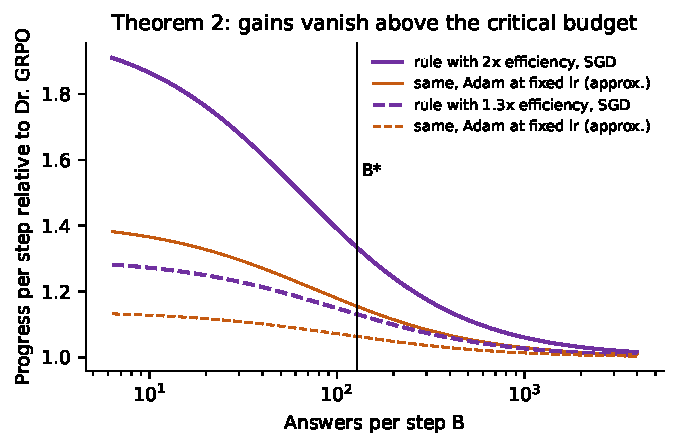
\includegraphics[width=0.5\linewidth]{regime.pdf}
\caption{Predicted gain of a better rule against answers per step: gains vanish above the critical budget, and Adam turns a gain of $k$ into about $\sqrt k$.}
\label{fig:regime}
\end{figure}

%=====================================================================
\section{Measuring the four numbers}\label{sec:measure}

\begin{why}
The theory's predictions depend on two unknowns: how $F_0$ compares with $F_1$, and how the learning signal $\|\nabla p\|^2$ varies with difficulty. Both had to be measured in a real model before any prediction meant anything.
\end{why}

\begin{found}
\textbf{Wrong answers carry larger gradients.} In Qwen2.5-Math-1.5B (exact per-answer gradients on MATH training problems): in the last-layer block, 40 questions by 16 answers, $F_1/F_0=0.36$ (90\% intervals do not overlap), while wrong answers are only 9\% longer (421 against 386 tokens). Over all 1.5B parameters, measured before every training run: $F_1/F_0$ between 0.32 and 0.42, so \textbf{wrong answers carry 2.4 to 3.1 times larger squared gradients}. Likely reason: wrong answers contain more low-probability tokens, whose scores are large. This contradicts VSR's Assumption B.3.

\textbf{The learning signal fades at both ends.} With 96 answers per question, the estimated $\|\nabla p\|^2$ is $0.73\pm0.60$ on very easy or very hard questions and $15.5\pm5.4$ on medium ones; the best fit is $p^2(1-p)^2$, and a flat shape is rejected (Figure~\ref{fig:shape}). This makes the optimal rule robust: it should spend answers on medium questions.
\end{found}

\begin{figure}[H]
\centering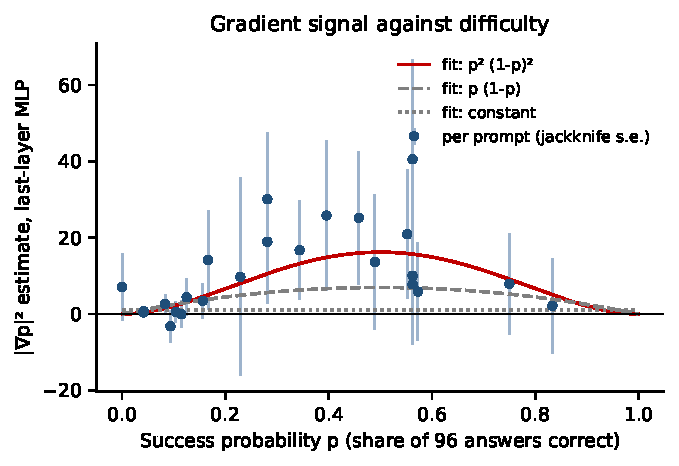
\includegraphics[width=0.5\linewidth]{shape.pdf}
\caption{Per-question learning signal against success probability, with three candidate shapes.}
\label{fig:shape}
\end{figure}

%=====================================================================
\section{First tests of the theory}

\subsection{Pre-registration 1: scale down wrong answers (pilot)}
\begin{why}
The simplest consequence of $F_0>F_1$: weight each wrong answer's advantage by $w=F_1/F_0$. A one-line change to Dr.\ GRPO, predicted to raise efficiency by 1.1 to 1.6 times in 11 of 12 settings.
\end{why}
\textbf{Design.} Qwen2.5-Math-1.5B base, 3,920 numeric MATH training problems (four subjects), 16 questions by 8 answers per step, 150 steps, 512-token answers, AdamW at $10^{-6}$; Dr.\ GRPO against the scaled version; two seeds; primary: greedy accuracy on the 364 numeric MATH-500 problems. \textbf{Prediction:} promising if at least $+2$ points in both seeds.
\begin{found}
No gain: 45.3\% against 47.5\% (seed 1), 44.0\% against 46.7\% (seed 2). Verdict: \textbf{no evidence}. Lesson: under Adam at a fixed learning rate, a 1.1 to 1.6 times efficiency gain shrinks to 1.06 to 1.25 times, too small to see with two seeds.
\end{found}

\begin{figure}[H]
\centering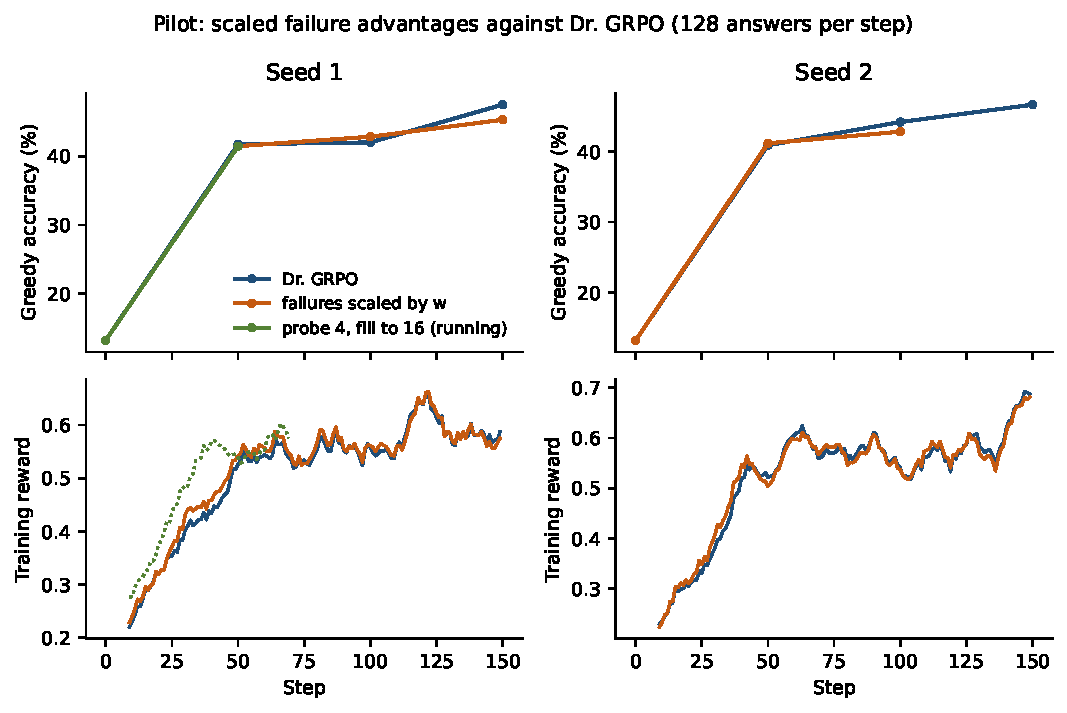
\includegraphics[width=0.8\linewidth]{pilot.pdf}
\caption{Pilot: scaled failures (orange) track Dr.\ GRPO (blue).}
\end{figure}

\subsection{Pre-registrations 2 and 3: collection rules at equal cost, and measuring noise inside training}
\begin{why}
The optimal rule predicts a larger gain (1.7 to 2.3 times Dr.\ GRPO's efficiency). Testing it fairly needs exactly matched generated answers. And to know \emph{why} a rule helps or not, we needed to measure signal and noise during training, not just accuracy.
\end{why}
\textbf{Design.} The optimal rule (lookup table re-solved every 10 steps from the recent difficulty mix), probe-then-fill, scaled failures, and Dr.\ GRPO at several budgets (32 to 256 answers per step), all at matched answers (19,200 over 150 steps for the 128-answer arms), two seeds, paired per problem on 3,382 held-out MATH test problems. \textbf{New tool:} at every step the questions are split at random into two halves; inner products of the two halves' gradients, and of each half with an independent unbiased reference for the population gradient, give the signal, the noise and the noise scale, without extra sampling. \textbf{Prediction:} promising if the optimal rule beats Dr.\ GRPO by at least 1.5 points in both seeds.
\begin{found}
\begin{itemize}[leftmargin=*,itemsep=1pt]
\item Optimal rule: $+1.1\pm0.4$ (seed 1) and $+3.3\pm0.5$ (seed 2) points, with matched answers (19,172 and 19,200) and about 1\% more tokens. Positive in both seeds, but the pre-registered bar (1.5 in both) was \textbf{missed} because of seed 1.
\item Probe-then-fill: $+2.0$ and $+0.8$ (MATH-500). Scaled failures: $-0.4$ and $+1.1$. Fewer answers clearly hurts: 32 against 128 answers per step, $-4.4$ points (seed 1; not every rung of the budget ladder obtained GPUs).
\item Training becomes noise-limited as it plateaus: Dr.\ GRPO's noise scale grows from about 900 answers (steps 0 to 49) to over 10,000 (steps 50 to 149): the shared signal shrinks while the noise does not.
\item Gains are much smaller than one-step theory predicts, consistent with Adam's square-root effect.
\end{itemize}
\end{found}

%=====================================================================
\section{The literature check and the change of direction}

\begin{why}
Before investing more, we checked carefully (three literature reviews, key claims verified by hand) whether the framing was new.
\end{why}
\begin{found}
\begin{itemize}[leftmargin=*,itemsep=1pt]
\item \textbf{The critical-budget framing was taken} (Bansal et al., HiLD at ICML 2026), including the finding that within-question noise dominates.
\item The common evaluation flaws listed in Section~\ref{sec:lit}.
\item \textbf{No paper measures gradient norms by correctness}, as far as we found, and none separates the average and the noise of positive and negative reinforcement.
\end{itemize}
\end{found}
So the main question moved to positive versus negative reinforcement, where our theorem and our measurement give something nobody else has. The optimal-rule result stays as a practical side result.

\subsection{The key observation}
Give each right answer advantage $a$ and each wrong answer $b$. The theorem gives
\[
\E g = n(a-b)\,\nabla p,\qquad \text{noise}\approx n\big(a^2pF_1+b^2(1-p)F_0\big).
\]
\begin{itemize}[leftmargin=*,itemsep=1pt]
\item PSR ($a=1,b=0$) and NSR ($a=0,b=-1$) both have average $n\nabla p$: \textbf{exactly the same expected update}. (This is the classical baseline invariance; the new part is the noise and its measurement.)
\item In fact NSR $=$ PSR $-\sum_i\nabla\log\pi(y_i)$, and the extra term has average exactly zero: it is pure noise.
\item PSR's noise $npF_1$ sits on easy questions; NSR's $n(1-p)F_0$ on hard ones. With $F_0\approx2.5F_1$, NSR is noisier on every question solved less than 71\% of the time.
\item The whole family $A=r-b$ shares the average; its noise is smallest near $b^\star=pF_1/(pF_1+(1-p)F_0)\approx0.15$.
\end{itemize}
\textbf{Consequence:} to first order, any difference between PSR and NSR (entropy, pass@$k$) must come from the noise, from an optimizer that reacts to noise (Adam), or from implementation choices outside the theorem.

%=====================================================================
\section{PSR against NSR (Pre-registration 4)}\label{sec:p4}

\begin{why}
Test the observation directly: if NSR's famous diversity advantage is real in clean on-policy training with equal averages, it must be a noise effect; if it does not appear, it must come from implementation.
\end{why}
\textbf{Design.} Dr.\ GRPO, PSR, NSR, W-REINFORCE; two seeds; strictly on-policy; in-training noise measurement; an on-policy entropy probe (the first four answers of every question, identical for all rules); pass@$k$ with 64 samples at step 150. \textbf{Prediction:} separation if NSR beats PSR by at least 3 points of pass@64, or has at least 20\% more entropy, in both seeds.

\begin{table}[H]
\centering\small
\resizebox{\linewidth}{!}{\begin{tabular}{@{}lcccc@{}}
\toprule
\textbf{Rule} (seed 1 / seed 2) & \textbf{Training acc., steps 25--49} & \textbf{pass@1 at 150} & \textbf{pass@64 at 150} & \textbf{Entropy, 100--150}\\
\midrule
Dr.\ GRPO & 50.6 / 48.0 & 43.3 / 43.2 & 83.2 / 81.9 & 0.227 / 0.224\\
PSR (reward right only) & 51.3 / 48.2 & 42.4 / 42.0 & 83.2 / 83.8 & 0.227 / 0.226\\
NSR (penalize wrong only) & 33.6 / 36.4 & 37.7 / 39.1 & 83.0 / 82.1 & 0.251 / 0.251\\
W-REINFORCE & 38.6 / 38.0 & 38.5 / 39.8 & 80.5 / 81.3 & 0.243 / 0.256\\
\bottomrule
\end{tabular}}
\caption{Untrained model: pass@1 13.8, pass@64 79.9.}
\end{table}

\begin{found}
NSR's measured noise is 6.4 times PSR's (theory about 7). NSR learns clearly more slowly, ends with lower pass@1, and reaches the \emph{same} pass@64; its entropy is only 11\% higher. The measured noise matches the theorem within 30\% for every rule. Verdict: \textbf{the separation is not reproduced} in either seed. W-REINFORCE, the NSR paper's recommendation, has the lowest pass@64.
\end{found}

\begin{figure}[H]
\centering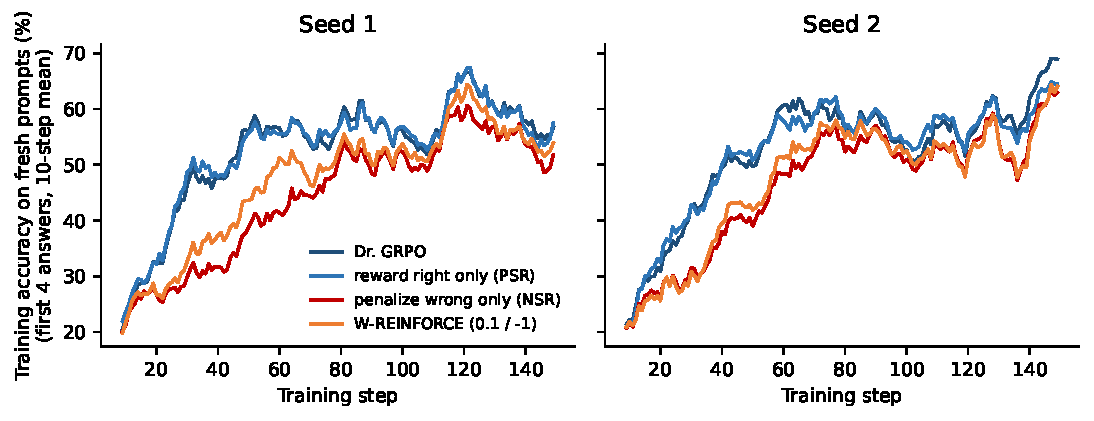
\includegraphics[width=0.85\linewidth]{pn_curves.pdf}
\caption{Training accuracy on fresh questions. The noisy rules, dominated by wrong answers, learn about twice as slowly.}
\end{figure}

\begin{figure}[H]
\centering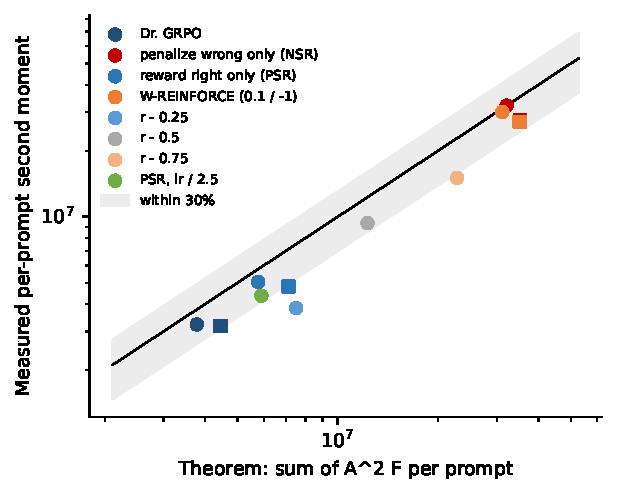
\includegraphics[width=0.45\linewidth]{noise_validation.pdf}
\caption{Measured gradient noise against the theorem's prediction from $F_0$, $F_1$ and the observed reward counts; shaded: within 30\%.}
\end{figure}

%=====================================================================
\section{Matched accuracy, and the NSR paper's own implementation}

\subsection{Pre-registration 5: is NSR just a slower PSR?}
\begin{why}
At a fixed step, a slower run looks more diverse simply because it has learned less. The fair comparison is diversity \emph{at the same accuracy}: for each NSR checkpoint, interpolate PSR's pass@32 at the same pass@1 along PSR's trajectory and take the difference. This gives an \textbf{accuracy-versus-diversity curve} per run.
\end{why}
\textbf{Design.} PSR and NSR, seeds 3 and 4, pass@32 from 32 samples on 128 MATH-500 problems at steps 0 to 150. \textbf{Prediction:} the matched difference is below 2 points in both seeds.
\begin{found}
NSR is 2.1 points \emph{below} PSR's curve (seed 3) and 0.2 below (seed 4). \textbf{No extra diversity at equal accuracy} (Figure~\ref{fig:frontier}, left).
\end{found}

\subsection{Pre-registration 6: do the NSR paper's implementation choices create the effect?}
\begin{why}
Zhu et al.\ used verl, which differs from clean training in three ways the theorem does not cover: each batch of answers is reused for 4 updates with clipping (stale samples), each answer's loss is averaged over its tokens, and PSR and NSR average over only the answers they train on. If the effect lives anywhere, it may live there.
\end{why}
\textbf{Design.} All three choices reproduced at matched answers and updates (with fresh samples, our clipped loss equals the plain loss exactly). \textbf{Prediction:} recreated if NSR beats PSR by 3 points of pass@32, or 20\% entropy, in both seeds.
\begin{found}
NSR learns even more slowly here (training accuracy 31.0 and 31.4 against 43.0 and 45.4), and at step 150 its pass@32 is 7.0 and 1.6 points \emph{lower} than PSR's; its entropy is 1.11 and 1.18 times PSR's; at matched pass@1 the differences are $+0.3$ and $-1.3$. Verdict: \textbf{not recreated}. Disclosure found later: per-token averaging makes gradients larger, so the gradient clipping at norm 1 (verl's default) was active on 26 to 28\% of NSR's steps and 7 to 8\% of PSR's; it never triggered in any other on-policy run.
\end{found}

\begin{figure}[H]
\centering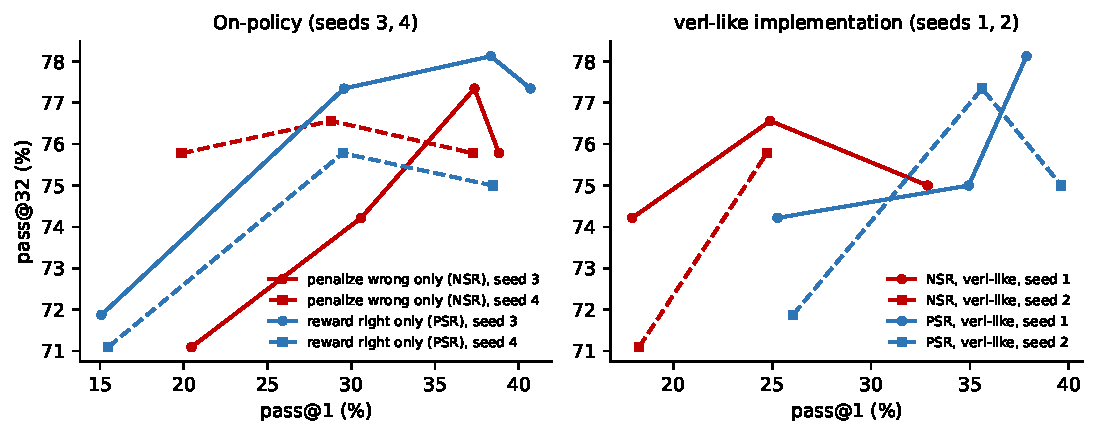
\includegraphics[width=0.95\linewidth]{frontier.pdf}
\caption{Accuracy (pass@1) against diversity (pass@32) during training, 128 problems. Left: changing the noise (PSR, NSR, PSR at a lower learning rate). Middle: the NSR paper's implementation. Right: changing the objective (pass@4 against Dr.\ GRPO). No run separates from its reference beyond the evaluation noise (point comparisons, not yet an equivalence test).}
\label{fig:frontier}
\end{figure}

%=====================================================================
\section{Same average, graded noise (Pre-registration 7)}

\begin{why}
The strongest test of ``only noise differs'' available with one family: the baselines $A=r-b$ for $b=0, 0.25, 0.5, 0.75, 1$ all have exactly the same average update, but the theory predicts different noise. If learning speed follows the predicted noise, noise is the likely cause. A PSR run with the learning rate divided by 2.5 tests the ``slower clock'' reading: does NSR look like PSR run more slowly?
\end{why}

\begin{table}[H]
\centering\small
\resizebox{\linewidth}{!}{\begin{tabular}{@{}lcccccc@{}}
\toprule
& $b=0.25$ & $b=0$ (PSR) & $b=0.5$ & $b=0.75$ & $b=1$ (NSR) & PSR, lr $/2.5$\\
\midrule
Predicted noise vs PSR & 0.81$\times$ & 1$\times$ & 1.25$\times$ & 2.5$\times$ & about 6$\times$ & 1$\times$\\
Steps to 45\% training accuracy, seed 3 & 37 & 44 & 44 & 53 & 56 & 84\\
Steps to 45\% training accuracy, seed 4 & 38 & 33 & 41 & 45 & 56 & 76\\
pass@32 vs PSR at equal pass@1, seed 3 & $+0.0$ & 0 & $+0.8$ & $-0.8$ & $-2.1$ & \\
pass@32 vs PSR at equal pass@1, seed 4 & $+0.2$ & 0 & $+2.1$ & $+0.6$ & $-0.2$ & \\
\bottomrule
\end{tabular}}
\end{table}

\begin{found}
\begin{itemize}[leftmargin=*,itemsep=1pt]
\item \textbf{Speed follows predicted noise} in both seeds (rank correlation 0.9 to 0.97; pre-registered threshold 0.8): passed.
\item The noise formula is within 30\% in all seed-4 runs but only 0.51 to 0.73 in seed 3, so 12 of 16 runs overall; likely because gradient sizes are measured once, before training, and shrink as the model sharpens.
\item Every run stays within about $\pm2$ points of PSR's curve; ``noise adds exploration'' is rejected. The strict slower-clock rule asked for every difference below 2 and two were 2.07 and 2.14: \textbf{formally inconclusive}. PSR at a 2.5 times lower learning rate learns \emph{more} slowly than NSR, so NSR equals a smaller slowdown.
\end{itemize}
\end{found}

%=====================================================================
\section{Changing the objective, and grading the reasoning (Pre-registration 8)}\label{sec:p8}

\begin{why}
If noise only changes speed, perhaps changing \emph{what the update aims at} moves the curve. We aimed the update exactly at pass@4: per-answer weights from the unbiased pass@$k$ estimator with a leave-one-out baseline, verified over all 256 reward patterns to average $2\cdot4(1-p)^3\nabla p$, the pass@4 gradient (such objectives are known, e.g.\ PKPO; here it is a control). It pushes hard questions and leaves solved ones alone. We also graded the reasoning, not just the final number, because a diversity gain could hide lucky guesses.
\end{why}
\textbf{Prediction:} the curve moves if pass@4 training is at least 2 points of pass@32 above Dr.\ GRPO at equal pass@1 in both seeds.
\begin{found}
$+1.6$ (seed 3) and $+0.2$ (seed 4): \textbf{curve fixed}. At step 150 pass@4 training simply has lower pass@1 (41 to 42 against 46). With reasoning graded by Claude Haiku 5.5 (three judgments per correct answer, majority vote; cost about \$9):
\begin{center}\small
\begin{tabular}{@{}lcccc@{}}
\toprule
Step 150, seed 3 / seed 4 & pass@1 & CoT-Pass@1 & pass@32 & CoT-Pass@32\\
\midrule
Dr.\ GRPO & 46.2 / 46.2 & 43.4 / 43.3 & 82.0 / 78.9 & 74.2 / 70.3\\
pass@4 objective & 41.2 / 42.3 & 38.6 / 39.3 & 78.9 / 81.2 & 72.7 / 72.7\\
Untrained model & 15.1 & 13.5 & 71.9 & 66.4\\
\bottomrule
\end{tabular}
\end{center}
Reasoning-checked diversity is the same (CoT-Pass@32 72.7 against 72.3 on average); about 93\% of trained models' correct answers have valid reasoning, up from 90\%.
\end{found}

%=====================================================================
\section{What the Qwen experiments say together}

\begin{idea}{The picture after eight pre-registrations}
In on-policy RLVR on Qwen2.5-Math-1.5B, every reward-shaping choice we tried (PSR, NSR, five baselines in between, the NSR paper's implementation, and a pass@4 objective) moved the model \emph{along} one accuracy-versus-diversity curve at different speeds; none moved the curve beyond about 2 points. The speed followed the noise that the theorem predicts from four numbers per question. NSR's ``preserved diversity'' is what any slower run looks like at a fixed step.
\end{idea}
Two side results: the theory explains why standard practice is close to right (Dr.\ GRPO's per-question baseline is 1.25 times less noisy than the best possible constant baseline), and the optimal answer-collection rule moves faster along the curve at equal cost. A planned method, WORTH-$k$ (a noise-minimized pass@$k$ objective), was dropped: it assumed that changing the objective moves the curve, and Pre-registration 8 found it does not at this scale.

%=====================================================================
\section{An independent review, and what we changed}

\begin{why}
The goal is an ICML paper. Before spending more, we asked an independent model (Codex) to review the project as a demanding ICML reviewer and area chair, and since then it reviews every experiment before launch.
\end{why}
\begin{found}
Verdict: \textbf{reject as it stands, 4 out of 10 (about 10 to 20\% acceptance), with a credible path to a main-track paper}; about 6 out of 10 (30 to 45\%) if a second model family establishes one curve with intervals; 5 out of 10 if the curves robustly differ. Its main points, all accepted:
\begin{enumerate}[leftmargin=*,itemsep=1pt]
\item \textbf{Novelty is narrower than framed.} Equal averages for PSR and NSR are classical baseline invariance; pass@$k$ objectives exist (PKPO); Dr.\ GRPO, the coverage framing (Yue et al.) and CoT-Pass@$k$ (Wen et al.) are prior work. Ours: the noise accounting with $F_0\neq F_1$ and adaptive group sizes, the measured asymmetry, and the matched-accuracy tests.
\item \textbf{``No difference detected'' was presented as ``the same''.} One 1.5B model, two seeds per comparison, 128 problems, point estimates; the NSR paper used 4B to 8B models and $k$ up to 256.
\item \textbf{Noise predicts speed, but cause is not shown.} The baseline family changes the noise and the push on wrong answers together.
\item Four numbers give the \emph{size} of the noise, not its geometry or what Adam does with it.
\end{enumerate}
\end{found}
\textbf{What we changed (no GPU needed):} the report, the collaborator brief and the story now credit baseline invariance and PKPO, drop every ``nobody measured this'' claim, describe the Qwen result as absence of detected separation, state the scale gap to the NSR paper, and disclose the clipping in Pre-registration 6. \textbf{What we launched:} the two experiments below, each reviewed by Codex several times (Pre-registration 9 four times, Pre-registration 10 three times) and changed after every review.

%=====================================================================
\section{A second model family (Pre-registration 9)}\label{sec:p9}
\begin{why}
Qwen2.5-Math reacts even to random rewards, so small effects on it are suspect. The claim had to hold on a different family, for longer training, with a larger evaluation and proper equivalence intervals rather than ``no difference seen''.
\end{why}
\textbf{Design.} OLMo-2-1B-SFT (AllenAI, never RL-trained), all seven MATH training subjects (5,685 problems), 300 steps, answers up to 1,024 tokens, five rules (Dr.\ GRPO, PSR, NSR, the pass@4 objective, the optimal collection rule) and two seeds; checkpoints every 50 steps evaluated with 32 samples on 256 held-out, subject-stratified problems; greedy accuracy on 3,382 test problems at the end.
\begin{found}
\begin{center}\small
\resizebox{\linewidth}{!}{\begin{tabular}{@{}lll@{}}
\toprule
Test & Result & Verdict\\
\midrule
Wrong answers have larger gradients & 2.14 [1.55, 2.93] and 2.54 [1.73, 3.65] & \textbf{passed}, both seeds\\
NSR noisier than PSR & 19.5$\times$ and 22.2$\times$ & \textbf{passed}\\
NSR slower to reach the midpoint & seed 1 tie (52 vs 52), seed 2 88 vs 41 & failed (needs both)\\
\textbf{NSR vs PSR, same curve (primary)} & $-0.30$, 90\% [$-1.28$, $+0.77$] & \textbf{equivalent within $\pm2$}\\
pass@4 objective vs Dr.\ GRPO & $+1.32$, 90\% [$+0.24$, $+2.26$] & inconclusive (a small lift)\\
Optimal rule vs Dr.\ GRPO, equal answers & $+0.65$ [$-0.24$, $+1.54$] & inconclusive\\
\bottomrule
\end{tabular}}
\end{center}
The main claim replicates on a second family: penalizing wrong answers lies on the same accuracy--diversity curve as rewarding right ones. No formatting flag; removing the one problem whose answer key was wrong changes nothing.
\end{found}
\begin{figure}[H]
\centering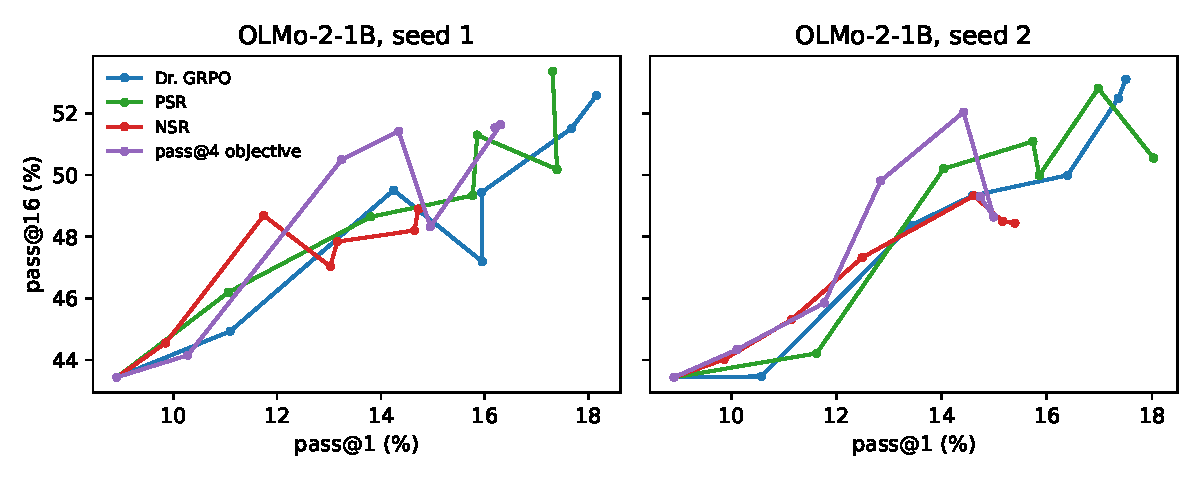
\includegraphics[width=0.85\linewidth]{olmo_curves.pdf}
\caption{OLMo: accuracy (pass@1) against diversity (pass@16) at steps 0 to 300. The rules lie on one curve.}
\end{figure}

\section{Is the noise the cause? (Pre-registration 10)}\label{sec:p10}
\begin{why}
The reviewer's main objection: noise \emph{predicts} learning speed, but in the baseline family more noise always came with a harder push on wrong answers, so the cause was not shown.
\end{why}
\textbf{The intervention.} Add to PSR a random-sign term whose size, at every step, matches NSR's predicted noise. It averages to zero, so the expected update is unchanged, and it never pushes wrong answers down systematically. If this ``PSR + noise'' learns as slowly as NSR, noise of that size is enough to cause NSR's lag. Three fresh seeds; also NSR and PSR at twice the learning rate; an NSR ``shadow'' computed on the same answers to check the noise really matches.
\begin{found}
\begin{itemize}[leftmargin=*,itemsep=1pt]
\item The noise matched: 1.02 [1.01, 1.05] times NSR's.
\item \textbf{PSR + noise is as slow as NSR}: speed $\phi=-0.11$ [$-0.22$, $-0.05$] on a scale where NSR is 0 and PSR is 1 (pre-registered margin $\pm1/3$; passed; one seed flagged).
\item NSR at twice the learning rate recovers its whole lag ($\phi=1.16$); at a matched doubled rate the gap shrinks to 31\%.
\item \textbf{Same curve}, now with intervals on Qwen: NSR vs PSR $-0.20$ [$-0.97$, $+0.55$], PSR + noise $-0.37$ [$-1.13$, $+0.46$], NSR at 2$\times$ $-0.03$ (all equivalent within $\pm2$).
\item The noise formula fits training within 0.69--1.18 once gradient sizes are re-measured (the asymmetry fades from about 3$\times$ to 1.5$\times$).
\item Adam: NSR's raw noise is 6$\times$ PSR's but only 1.0--1.3$\times$ after Adam's scaling; NSR's steps point 13--27\% less along the true improvement direction. Noise does not shrink Adam's steps, it misdirects them.
\end{itemize}
\end{found}
\begin{figure}[H]
\centering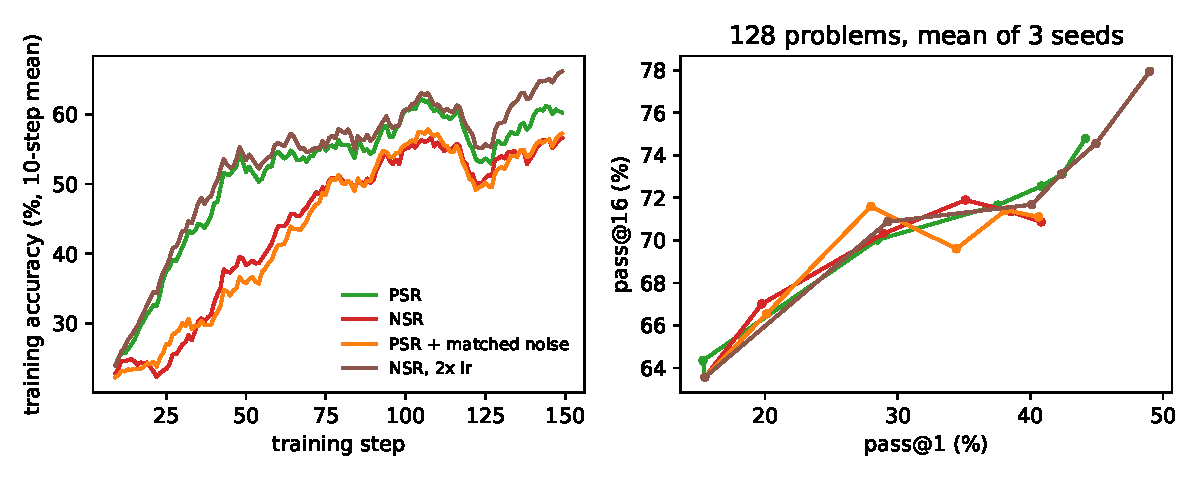
\includegraphics[width=0.85\linewidth]{noise_test.pdf}
\caption{Left: training accuracy; PSR + matched noise (orange) learns as slowly as NSR (red); NSR at twice the learning rate (brown) as fast as PSR (green). Right: all four lie on one accuracy--diversity curve.}
\end{figure}

\section{Is the curve a temperature effect? (Pre-registration 11)}\label{sec:p11}
\begin{why}
By our proposition, diversity at matched accuracy is how evenly success is spread over questions. If RL simply made the model globally more confident (like lowering the temperature), then sampling a late checkpoint at a higher temperature should beat the training curve, and a method that limits sharpening would have room to work. This decides which method to build.
\end{why}
\textbf{Design.} The PSR checkpoints of Pre-registration 10 and the base model, sampled at temperatures 0.5 to 1.6; the quantity $D$ is the late checkpoint's pass@16 at a raised temperature minus the training trajectory's pass@16 at the same pass@1. The model's entropy is also measured on fixed base-model answers.
\begin{found}
\begin{itemize}[leftmargin=*,itemsep=1pt]
\item \textbf{RL does not sharpen globally.} On fixed text the entropy barely changes (1.081 for the base, 1.064 after training), while on the model's own samples it falls three- to fourfold: RL steers into confident paths.
\item \textbf{Undoing sharpening does not help.} At the temperature that restores the base entropy ($T^\ast=1.01$), $D=0.0$ in every seed; slightly higher temperatures stay on the curve; at 1.3 formatting breaks and coverage falls. Pre-registered verdict: inconclusive ($D=-1.54$ on 256 problems; $-1.42$, 90\% [$-2.19$, $-0.68$], on 511).
\item RL is far above anything temperature does for the base model ($+7$ to $+16$ points): RL adds ability, not only sharpening.
\end{itemize}
\textbf{Consequence (declared in advance):} the memory branch of the method experiment runs.
\end{found}
\begin{figure}[H]
\centering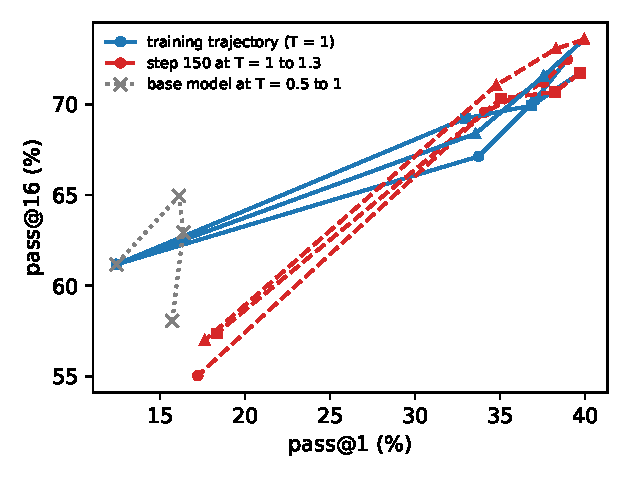
\includegraphics[width=0.5\linewidth]{temperature.pdf}
\caption{Training trajectory (blue), the late checkpoint at higher temperatures (red), and the base model at lower temperatures (gray).}
\end{figure}

\section{Checking the answer keys}
\begin{why}
An independent review found two wrong reference answers in the evaluation sets. Before using them to judge a method, every answer had to be checked.
\end{why}
\begin{found}
Claude Haiku 5.5 solved all 768 evaluation and validation problems; where it disagreed with the key, Claude Opus 5.5 adjudicated. \textbf{3 of 768 keys were wrong (0.4\%)}: a sign error (corrected) and two questions with several answers whose key kept one (excluded). They affect all methods equally; excluding the one in the OLMo set changes no verdict.
\end{found}

\section{From diagnosis to method (Pre-registration 12)}\label{sec:p12}
\subsection{What the diagnosis says a method must do}
\begin{center}\small
\begin{tabularx}{\linewidth}{@{}P{0.46\linewidth}Y@{}}
\toprule
\textbf{Diagnostic finding} & \textbf{Requirement for a method}\\
\midrule
Correctness-only rules (PSR, NSR, baselines, pass@$k$ weights, adaptive sampling) only reweight questions and change noise; they share one curve & Bring in information the current samples do not contain\\
Diversity at matched accuracy = how evenly success is spread across questions & Raise success on rarely solved questions without hurting solved ones\\
On rarely solved questions a group of 8 is usually all wrong, and the signal fades as $p^2(1-p)^2$ & Supply signal exactly there\\
RL does not sharpen globally; entropy control blocks learning & Do not regulate entropy\\
Extra noise slows learning & Keep Dr.\ GRPO's low-noise update as the base\\
\bottomrule
\end{tabularx}
\end{center}

\subsection{The method: coverage-weighted success replay}
\begin{idea}{Coverage-weighted memory (CM)}
Train with Dr.\ GRPO as usual. Store every verified, completed, distinct correct answer the model finds (at most 4 per question). Each step, replay 8 stored questions by adding the gradient of $\lambda\sum_q\log\sum_{y\in S_q}\pi(y\mid q)$, choosing questions in proportion to the expected value of $k\,p(1-p)^{k-1}$ ($k=16$, $p$ the question's estimated success rate). This weight is exactly $\partial\,\mathrm{pass@}k/\partial\log p$: replay goes to questions solved about one time in $k$, whose pass@$k$ can still rise, not to questions already solved.
\end{idea}
Plain replay of stored successes is known (MAPO, self-imitation, STaR, RAFT, ReST); the new parts are the derivation from the diagnosis and the coverage weighting, so uniform replay (M) is run as the ablation at the same strength. Audit arms: the published unlikeliness reward (U), entropy bonus (E), adaptive entropy control (A), and, for the other branch, an entropy floor on the first 32 tokens of each answer (EF).

\subsection{The pilot (one seed, 100 steps, 255 validation problems)}
\begin{center}\small
\resizebox{\linewidth}{!}{\begin{tabular}{@{}lccc@{}}
\toprule
Arm & pass@1 & pass@16 & gain at matched accuracy\\
\midrule
Dr.\ GRPO, steps 0 / 50 / 100 & 15.1 / 35.5 / 39.3 & 63.9 / 71.1 / 72.5 & reference\\
\textbf{Coverage memory, $\lambda=1$ (chosen)} & 35.8 & 73.3 & \textbf{$+2.1$}\\
Coverage memory, $\lambda=4$ & 33.1 & 70.2 & $0.0$\\
Uniform memory, $\lambda=1$ & 38.6 & 72.4 & $+0.2$\\
Uniform memory, $\lambda=4$ & 35.3 & 74.2 & $+3.2$ (4 points slower; excluded by the rule)\\
Entropy bonus & 38.9--39.6 & 72.6--72.7 & about 0\\
Unlikeliness reward & 38.7 & 71.7 & about $-0.5$\\
Adaptive entropy & 9.3--25.5 & 48.9--65.0 & $-2.5$ or collapsed\\
Early-token entropy floor & 12.6--12.8 & 56.1--58.6 & collapsed (below the base model)\\
\bottomrule
\end{tabular}}
\end{center}
\textbf{Reading.} Memory is the only family that lifts the curve; at the same strength, coverage weighting gives $+2.1$ against $+0.2$ for uniform replay (one seed, noise about $\pm2$). Entropy-based fixes do not help or break learning, as the diagnosis predicted.

\subsection{The main runs (running)}
Seeds 8, 9, 10; Dr.\ GRPO, coverage memory, uniform memory and the unlikeliness reward, run in parallel on one 4-GPU machine per seed, 150 steps; evaluation on 511 held-out problems with 32 samples at steps 50, 100, 150, Dr.\ GRPO also at raised temperatures, and greedy accuracy on 3,382 test problems. Pre-registered rules: coverage memory \textbf{moves the curve} if it is at least 2 points above Dr.\ GRPO's curve, \emph{including the best temperature for Dr.\ GRPO}, with a 95\% interval above 0, in all three seeds, and confirmed on the 256 problems never used before; \textbf{coverage weighting matters} if it beats uniform memory by at least 1 point with a 95\% interval above 0; its accuracy at equal compute is reported separately.

\section{Where we stand, and the path to ICML}
\subsection{The independent review over time}
\begin{center}\small
\resizebox{\linewidth}{!}{\begin{tabular}{@{}lll@{}}
\toprule
When & Score (Codex as ICML reviewer) & Why it changed\\
\midrule
After the Qwen experiments & 4/10 & claims too broad; equivalence and cause not shown\\
After the noise-only test & 5/10 & noise shown to cause the lag\\
After OLMo & 6/10 (weak accept) & same curve on a second family, with intervals\\
Target & 7/10 & a method that moves the curve, beyond plain replay, replicated on OLMo\\
\bottomrule
\end{tabular}}
\end{center}

\subsection{The paper}
\begin{idea}{Claim}
In on-policy RLVR, reward shaping that uses only correctness changes \emph{how fast} a model moves along an accuracy--diversity curve, not the curve: positive and negative reinforcement share their expected update and differ in noise, which wrong answers dominate. Diversity at matched accuracy is how evenly success is spread across questions, so moving the curve needs information on rarely solved questions; coverage-weighted replay of verified successes supplies it. \textcolor{red}{[last sentence pending the main runs]}
\end{idea}

\subsection{Outcomes}
\begin{center}\small
\begin{tabularx}{\linewidth}{@{}P{0.42\linewidth}Y@{}}
\toprule
Main runs & Paper\\
\midrule
Coverage memory moves the curve and beats uniform replay; replicates on OLMo & Diagnosis plus a derived method: the 7/10 case\\
Memory moves the curve, but weighting does not matter & Diagnosis plus ``replay is what moves the curve, and here is why'': about 6--6.5/10\\
Nothing moves the curve & Diagnostic paper with a strong negative audit: about 6/10\\
\bottomrule
\end{tabularx}
\end{center}

\subsection{Timeline}
Main runs: about 3 hours of training and 4 of evaluation, then the analysis and an independent review. If positive: the OLMo replication (Pre-registration 13, about one day, reusing the existing OLMo Dr.\ GRPO runs). Then the ICML draft (already started, \texttt{paper/icml/}), with a larger model as an option if time allows (deadline usually late January).

\subsection{Cost}
Roughly \$1,500--2,000 so far across all experiments on SageMaker, plus about \$30 of LLM judging and auditing; the main method runs add about \$350--450.

\appendix
\section{Experiment tracker}\label{app:tracker}
\small
\begin{longtable}{@{}P{0.5cm}P{2.6cm}P{3.2cm}P{3.6cm}P{4.2cm}@{}}
\toprule
\textbf{\#} & \textbf{Question} & \textbf{Why} & \textbf{Design and prediction} & \textbf{Result and verdict}\\
\midrule
\endhead
S & STOP: do token-gradient interactions change the best cut? & Basis of a geometry-aware credit method & Exact per-token gradients, all partitions of a 64-token grid & Interactions tiny; best cut never changed. \textbf{Idea dropped}\\
\midrule
M & Do right and wrong answers have different gradient sizes? & The theory's predictions hinge on it & Exact per-answer gradients, last layer and full model & Wrong answers 2.4 to 3.1$\times$ larger squared gradients. \textbf{Established}\\
\midrule
M & How does the learning signal vary with difficulty? & Shapes the optimal rule & 96 answers per question & Fades at both ends ($p^2(1-p)^2$). \textbf{Established}\\
\midrule
1 & Does scaling down wrong answers help? & Simplest consequence of the asymmetry & Dr.\ GRPO vs scaled, 2 seeds; $\ge2$ points in both & $-2.2$, $-2.7$. \textbf{No evidence}\\
\midrule
2 & Optimal rule and probe-then-fill at equal answers & Theory predicts 1.7--2.3$\times$ efficiency & Matched answers; $\ge2$ points & Probe $+2.0$, $+0.8$; optimal moved to 3\\
\midrule
3 & When does collection matter? Measured noise & Explain gains or their absence & Budget ladder, optimal rule, in-training noise; $\ge1.5$ in both & Optimal $+1.1\pm0.4$, $+3.3\pm0.5$ (\textbf{threshold missed}); fewer answers $-4.4$; noise scale 900 $\to$ 10,000+\\
\midrule
4 & PSR vs NSR vs Dr.\ GRPO vs W-REINFORCE & Same average; is NSR's effect a noise effect? & 2 seeds, on-policy; $\ge3$ pass@64 or $\ge20\%$ entropy & pass@64 equal; NSR 6.4$\times$ noisier, slower. \textbf{Not reproduced}\\
\midrule
5 & Same diversity at equal accuracy? & Fixed-step comparisons confuse speed and diversity & Matched pass@1, seeds 3, 4; $|\text{diff}|<2$ & $-2.1$, $-0.2$. \textbf{No extra diversity}\\
\midrule
6 & Do the NSR paper's implementation choices create it? & Reuse, clipping, token averaging are outside the theorem & verl-like, 2 seeds; $\ge3$ pass@32 or $\ge20\%$ entropy & NSR $-7.0$, $-1.6$ at step 150. \textbf{Not recreated} (clipping active, disclosed)\\
\midrule
7 & Does speed follow predicted noise? & Same average, graded noise & 5 baselines + PSR at lr/2.5, 2 seeds; rank corr.\ $\ge0.8$ & 0.9--0.97, \textbf{passed}; slower clock \textbf{inconclusive} (2.07, 2.14)\\
\midrule
8 & Does changing the objective move the curve? & Test the other half of the principle & pass@4 vs Dr.\ GRPO, 2 seeds; $\ge2$ & $+1.6$, $+0.2$, CoT-Pass@32 equal. \textbf{Curve fixed}\\
\midrule
R & Is it an ICML paper? & Independent check before spending more & Codex as ICML reviewer & 4/10; corrections made; P9, P10 designed\\
\midrule
9 & Does it hold on OLMo, longer, with intervals? & Generality; Qwen is suspect for small effects & 5 rules, 2 seeds, 300 steps, 256 problems, equivalence $\pm2$ & NSR vs PSR $-0.30$ [$-1.28$, $+0.77$]: \textbf{equivalent}; asymmetry passed; speed rule failed (tie); pass@4 and optimal rule inconclusive\\
\midrule
10 & Is the noise the cause? & Causal test asked by the review & PSR + matched noise, NSR$\times$2, PSR$\times$2, 3 fresh seeds; $\phi$ within $\pm1/3$ & $\phi=-0.11$: \textbf{passed}; curves equivalent; Codex 5/10, then 6/10 with OLMo\\
\midrule
11 & Is the curve a temperature effect? & Decide the method branch & Late checkpoints at raised temperature vs the training trajectory & \textbf{Inconclusive} on 256 and 511 problems ($D=-1.42$); entropy on fixed text unchanged; RL $\gg$ base at any temperature $\to$ memory branch\\
\midrule
L & Are the answer keys right? & Two errors spotted & LLM solve plus adjudication, 768 problems & 3 wrong (0.4\%); corrected or excluded\\
\midrule
12p & Pilot: which strength? & Fix settings before the main runs & 12 arms, 1 seed, validation set & Coverage memory $\lambda=1$: $+2.1$; uniform $+0.2$; entropy fixes flat or collapsed\\
\midrule
12 & Does coverage-weighted memory move the curve? & The method derived from the diagnosis & 4 arms, 3 fresh seeds, 511 problems, Dr.\ GRPO envelope, untouched-half confirmation & \textbf{Running}\\
\bottomrule
\end{longtable}
\normalsize

\section{Glossary}
\begin{description}[leftmargin=*,itemsep=1pt,font=\normalfont\bfseries]
\item[Advantage] The weight that pushes a sampled answer up (positive) or down (negative).
\item[Baseline] A number subtracted from rewards; a constant one leaves the average update unchanged and changes the noise.
\item[Calibration] Measuring $F_0$ and $F_1$ on held-out questions before training.
\item[CoT-Pass@$k$] pass@$k$ counting only answers whose reasoning is judged valid.
\item[Critical budget / noise scale] The number of answers per step beyond which noise stops limiting progress.
\item[Dr.\ GRPO] Group-based RL with the group mean as baseline and no extra normalizations.
\item[$F_0$, $F_1$] Average squared gradient size of a wrong and of a right answer.
\item[Matched accuracy] Comparing diversity of two runs at the same pass@1, by interpolating along one run's trajectory.
\item[NSR, PSR] Penalize only wrong answers; reward only right answers.
\item[On-policy] Answers always come from the current model, one update per batch.
\item[pass@$k$] Share of questions with at least one right answer among $k$ samples.
\item[Pre-registration] A dated file fixing design, prediction and decision rule before the run.
\item[Score] $\nabla\log\pi(y)$: the direction that makes answer $y$ more likely.
\item[Split-half diagnostics] Splitting each step's questions into halves to measure the update's signal and noise in training.
\end{description}

\section{How we work, and engineering problems fixed}
\textbf{Method.} Every experiment: pre-registered; compared at matched generated answers; paired per problem; at least two seeds; an independent review (Codex) before launch since October 18; results reported whether they support the idea or not (most early predictions failed, and that shaped the project).

\textbf{Engineering issues fixed along the way.} GPU out-of-memory during evaluation (gradients kept alive; fixed by freeing them after each update); crashes on long held-out prompts (generation batch now capped by prompt length; the final check of Pre-registration 4 was lost); Hugging Face rate limits from shared AWS addresses (models now loaded from our S3 copy); a grader crash on a sampled \verb|\boxed{1/0}| (fixed and tested); a job wrapper that reported success when a run failed (fixed); GPU capacity shortages (each job launched in several regions at once, keeping the first to start). All code, pre-registrations, results and figures: \texttt{github.com/mayman150/rlvr-adaptive}.

\end{document}
